%%%%%%%%%%%%%%%%%%%%%%%%%%%%%%%%%%%%%%%%%
% Beamer Presentation
% LaTeX Template
% Version 1.0 (10/11/12)
%
% This template has been downloaded from:
% http://www.LaTeXTemplates.com
%
% License:
% CC BY-NC-SA 3.0 (http://creativecommons.org/licenses/by-nc-sa/3.0/)
%
%%%%%%%%%%%%%%%%%%%%%%%%%%%%%%%%%%%%%%%%%

%----------------------------------------------------------------------------------------
%	PACKAGES AND THEMES
%----------------------------------------------------------------------------------------

\documentclass{beamer}

\mode<presentation> {

% The Beamer class comes with a number of default slide themes
% which change the colors and layouts of slides. Below this is a list
% of all the themes, uncomment each in turn to see what they look like.

\usetheme{default}
%\usetheme{AnnArbor}
%\usetheme{Antibes}
%\usetheme{Bergen}
%\usetheme{Berkeley}
%\usetheme{Berlin}
%\usetheme{Boadilla}
%\usetheme{CambridgeUS}
%\usetheme{Copenhagen}
%\usetheme{Darmstadt}
%\usetheme{Dresden}
%\usetheme{Frankfurt}
%\usetheme{Goettingen}
%\usetheme{Hannover}
%\usetheme{Ilmenau}
%\usetheme{JuanLesPins}
%\usetheme{Luebeck}
%\usetheme{Madrid}
%\usetheme{Malmoe}
%\usetheme{Marburg}
%\usetheme{Montpellier}
%\usetheme{PaloAlto}
%\usetheme{Pittsburgh}
%\usetheme{Rochester}
%\usetheme{Singapore}
%\usetheme{Szeged}
%\usetheme{Warsaw}

% As well as themes, the Beamer class has a number of color themes
% for any slide theme. Uncomment each of these in turn to see how it
% changes the colors of your current slide theme.

%\usecolortheme{albatross}
%\usecolortheme{beaver}
%\usecolortheme{beetle}
%\usecolortheme{crane}
%\usecolortheme{dolphin}
%\usecolortheme{dove}
%\usecolortheme{fly}
%\usecolortheme{lily}
%\usecolortheme{orchid}
%\usecolortheme{rose}
%\usecolortheme{seagull}
%\usecolortheme{seahorse}
%\usecolortheme{whale}
%\usecolortheme{wolverine}

%\setbeamertemplate{footline} % To remove the footer line in all slides uncomment this line
%\setbeamertemplate{footline}[page number] % To replace the footer line in all slides with a simple slide count uncomment this line

%\setbeamertemplate{navigation symbols}{} % To remove the navigation symbols from the bottom of all slides uncomment this line
}
\usepackage{bbm}
\usepackage{graphicx} % Allows including images
\usepackage{booktabs} % Allows the use of \toprule, \midrule and \bottomrule in tables

%----------------------------------------------------------------------------------------
%	TITLE PAGE
%----------------------------------------------------------------------------------------

\title[Short title]{Masters Project} % The short title appears at the bottom of every slide, the full title is only on the title page

\author{Emily Palmer} % Your name
\institute[OSU] % Your institution as it will appear on the bottom of every slide, may be shorthand to save space
{
Group Meeting, Oregon State University  %\\ % Your institution for the title page
%\medskip
%\textit{john@smith.com} % Your email address
}
\date{\today} % Date, can be changed to a custom date

\begin{document}

\begin{frame}
\titlepage % Print the title page as the first slide
\end{frame}


\begin{frame}
  \frametitle{Motivation}
  
\includegraphics[width = \textwidth]{title.png}
\end{frame}

\begin{frame}
  \frametitle{Overview of Model}
  \begin{itemize}
    \item Correlation structure from taxonomic information
    \item Correlation structure from longitudinal data or repeated measures
    \item Two part model, using generalized estimating equations for parameter estimation
    \begin{itemize}
      \item Presence/Absence
      \item Relative Abundance of positive counts
    \end{itemize}
    \item Results from paper show this method to have accurate Type I error, unbiased estimation of model parameters, and more powerful than some existing methods.
  \end{itemize}
\end{frame}

\begin{frame}
  \frametitle{Application in paper}
  \begin{itemize}
    \item Twin obesity data Turnbaugh et. al. (2009)
    \item 54 families (clusters), 2 twins each, 2 time points
    \item Observations for 9 OTUs (only order Clostridiales)
    \item Obesity indication for each twin
    \item Some clusters are incomplete
  \end{itemize}
\end{frame}


\begin{frame}
\frametitle{Correlation matrix of taxonomic structure}
\begin{itemize}
  \item Assume that OTUs that belong to the same taxa at a higher level have some correlation
\end{itemize}
\begin{columns}[c] % The "c" option specifies centered vertical alignment while the "t" option is used for top vertical alignment

\column{.5\textwidth} % Left column and width
\textbf{Taxonomic structure}
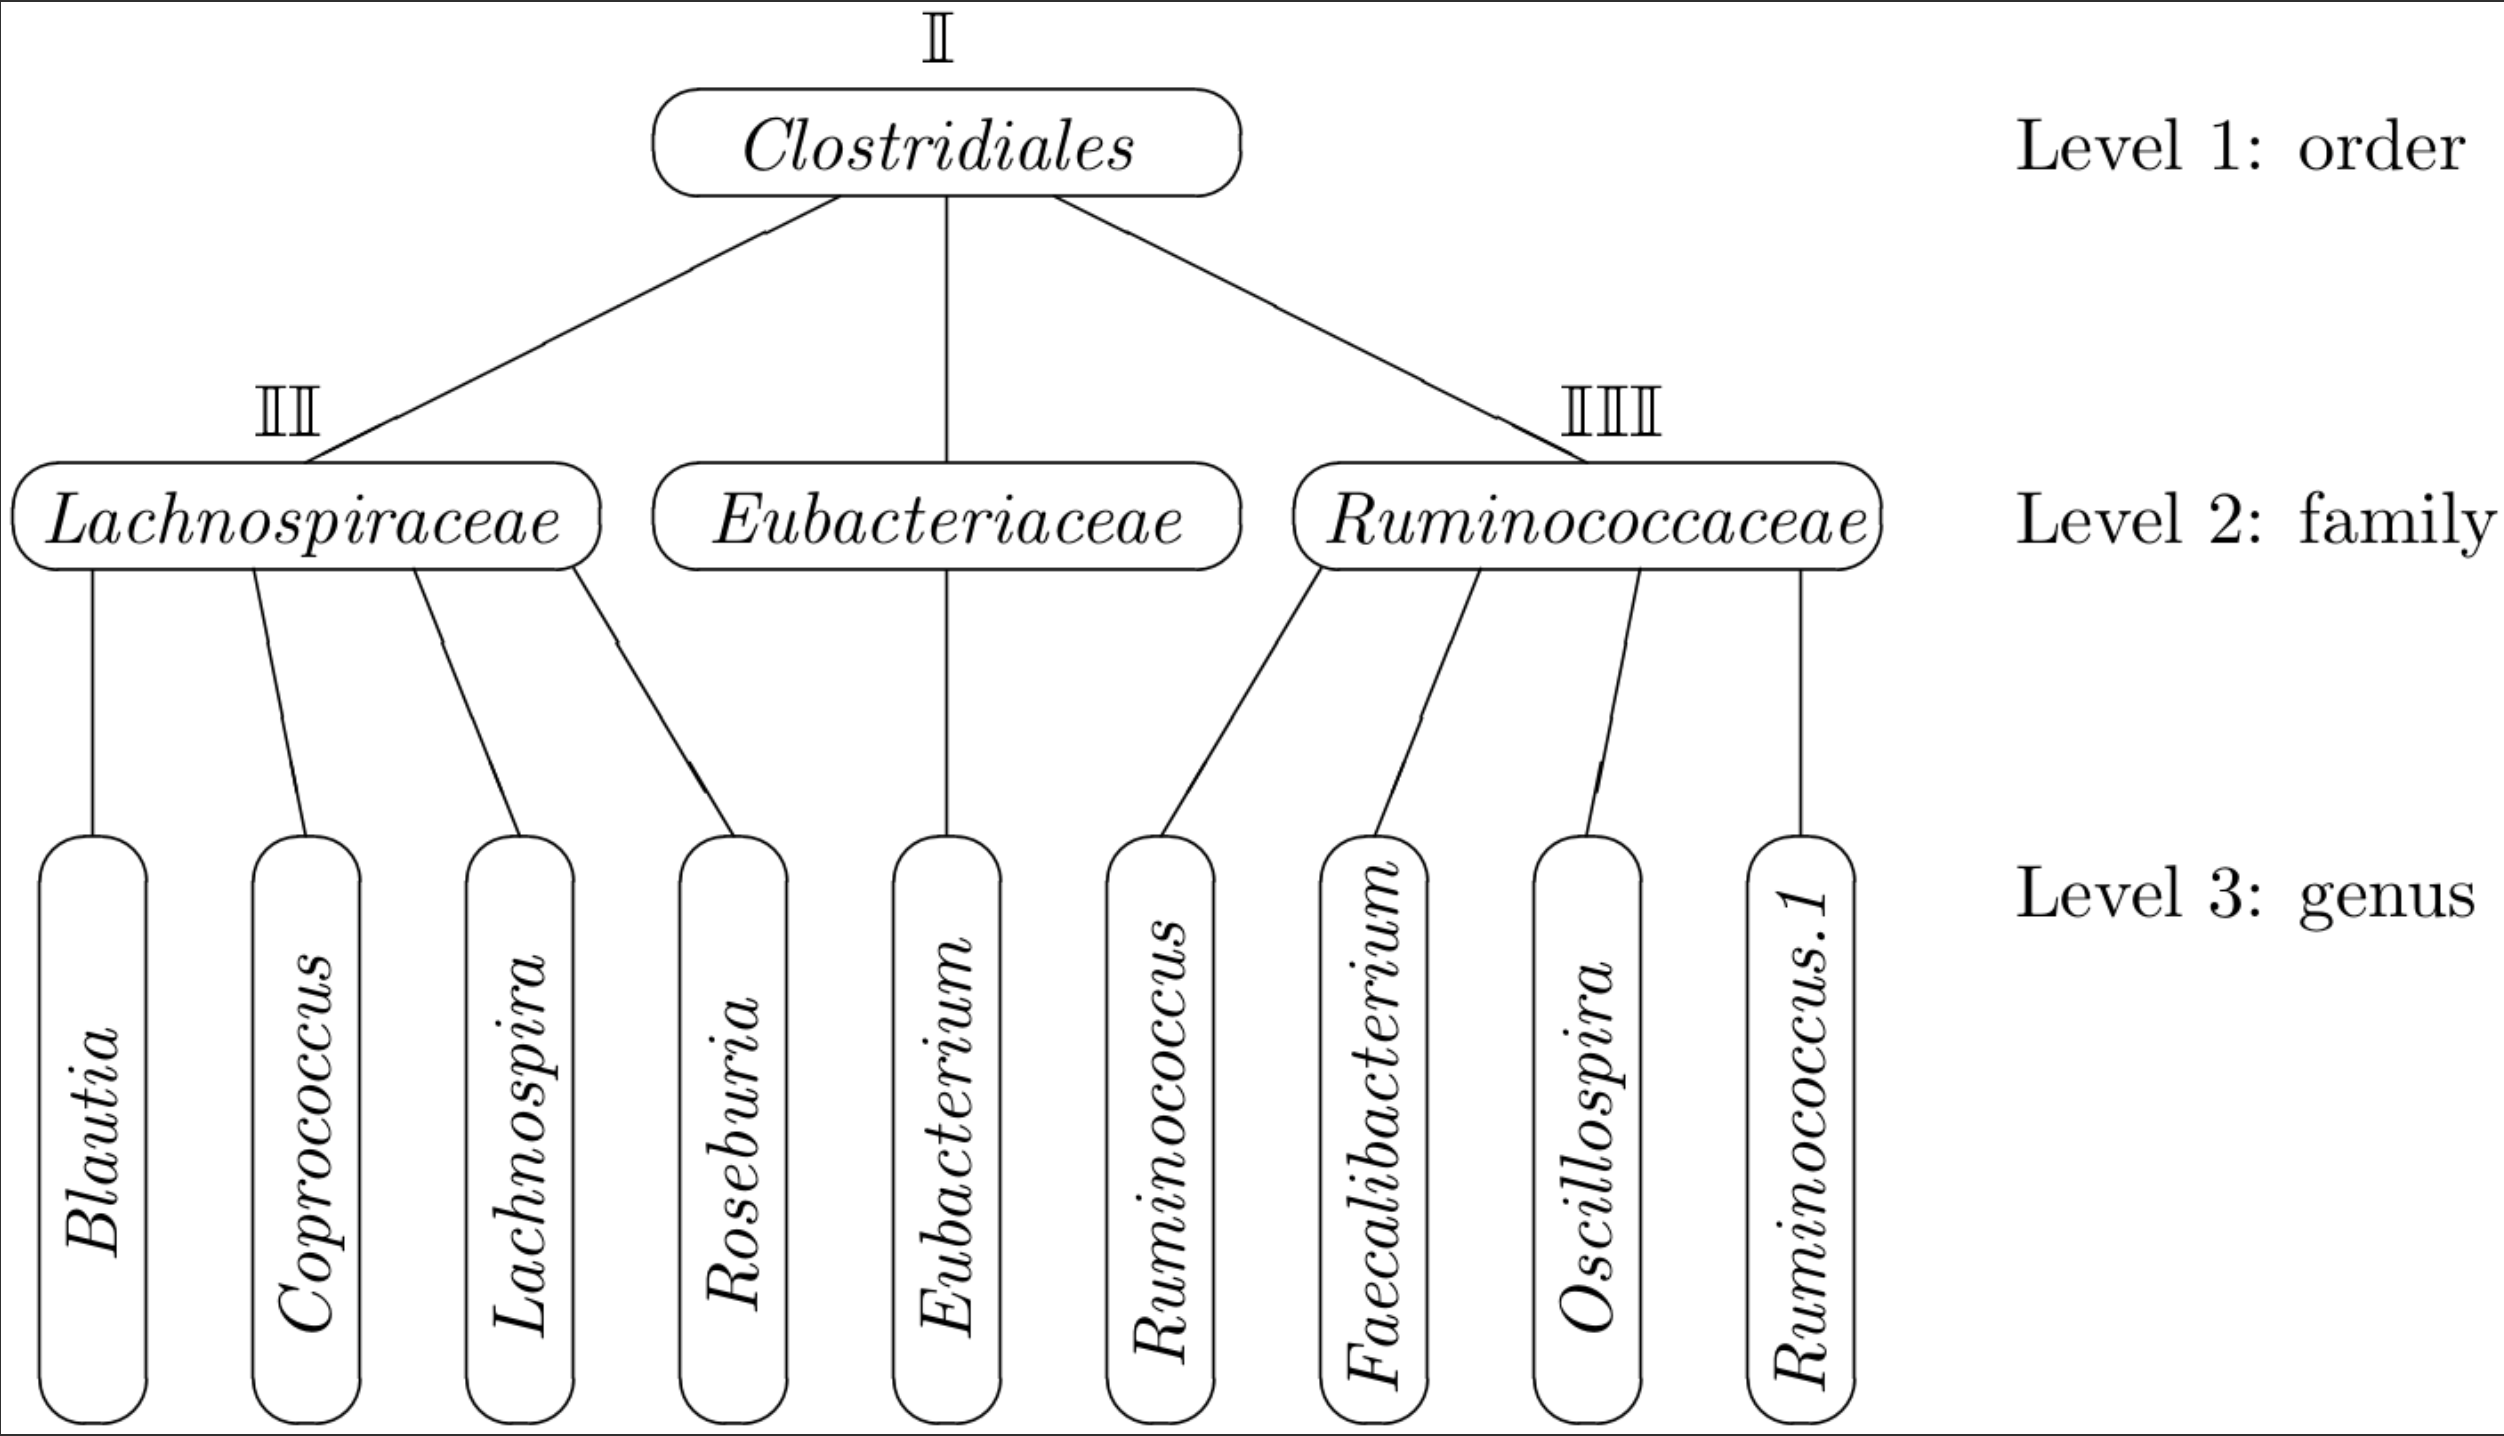
\includegraphics[width = \textwidth]{tax_tree.png}

\column{.5\textwidth} % Right column and width
\textbf{Gamma matrix}
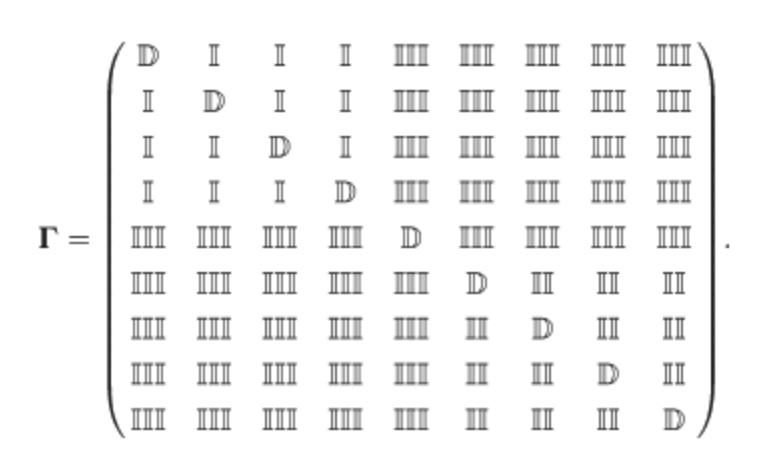
\includegraphics[width = \textwidth]{gamma.png}
\end{columns}
\end{frame}

\begin{frame}
  \frametitle{Combining with Longitudinal/Repeated Measure data}
  \begin{itemize}
    \item Correlation matrix for repeated measures - structure flexible
    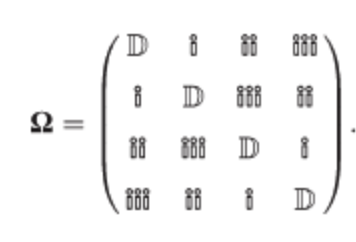
\includegraphics[width = .3\textwidth]{twin_omega.png}
    \item Integrative correlation matrix - This will be a block matrix indicating the distinct correlations of all combinations of time points and OTUs
    \item If $N$ is the number of OTUs, and $M$ the number of repeated measures, this integrative correlation matrix will have dimension $(N \times M) \times(N \times M)$
    \item This grows very quickly
  \end{itemize}
\end{frame}


\begin{frame}[t]{Working correlation matrix in R}
  \begin{itemize}
    \item The package \texttt{geepack} estimates the regression and covariance parameters
    \item Requires a specified working correlation matrix that is $\binom{N \times M}{2} \times  \text{ number correlation parameters}$ for one cluster
    \item For $n$ clusters, this will have dimension $\bigg(n \times \binom{N \times M}{2}\bigg) \times  \text{ number correlation parameters}$
    \item Correlations are linear combinations of the columns of the covariates based on the upper triangular part of the integrative correlation matrix.
  \end{itemize}
\end{frame}
%--- Next Frame ---%

\begin{frame}[t]{Adjusting for Incomplete Clusters}
  \begin{itemize}
    \item If we have the same number of observations per cluster, the working correlation matrix will be the same for each cluster
    \item Often, there will be some missing data for a cluster, missing time points, etc.
    \item The corresponding row and column of the integrative correlation matrix needs to be removed. This adjustment needs to be made for each cluster
    \item Corresponding rows of the working correlation matrix will need to be removed to run the code.
  \end{itemize}
\end{frame}
%--- Next Frame ---%



% \begin{frame}
%   \frametitle{Parameter estimation - GEEs }
%   here
% \end{frame}

\begin{frame}[t]{Scaling the model}

\end{frame}

\begin{frame}[t]{Scaling the model}
  \begin{itemize}
    \item Paper focused on data with only 9 OTUs
    \item How does this scale to a dataset with more common numbers of OTUs ($>1000$?)
    \item Focus currently only on taxonomic correlation aspect
  \end{itemize}
\end{frame}

\begin{frame}[t]{Scaling the model}
 \begin{itemize}
   \item As-is, this method does not scale well to larger datasets
 \end{itemize}
\end{frame}

\begin{frame}{American Gut data}
  \begin{itemize}
    \item Focus at genus level at one body sample site
    \item ~14300 taxa and
    \item ~260 correlation parameters to estimate
    \item Integrative correlation matrix will have dimension $14300 \times 14300$
    \item Working correlation matrix will have dimension $\binom{14300}{2} \times 240$ for one cluster
    \item Matrix is too large for R
  \end{itemize}
\end{frame}

\begin{frame}{Filter more?}
  \begin{itemize}
    \item Filter taxa based on threshold of genus sparsity
    \item Reduces to ~1200 taxa and
    \item ~72 correlation parameters to estimate.
    \item Integrative correlation matrix will have dimension $1200 \times 1200$
    \item Working correlation matrix will have dimension $\binom{1200}{2} \times 240$ for one cluster
    \item $\bigg(3000\times \binom{1200}{2}\bigg) \times 240$ for all clusters
    \item Matrix is again too large for R
  \end{itemize}
\end{frame}


\begin{frame}[t]{Discussion}
  \begin{itemize}
    \item Better ways to scale this model?
    \item Another implementation of fitting GEEs in R? 
    \item Focus on groups of OTUs individually?
    \item Would aggregating to a higher taxa level help?
    \item American Gut covariates to use?
  \end{itemize}
\end{frame}
%--- Next Frame ---%




% \begin{frame}[t]{GEE Model for OTUs}
%   \begin{itemize}
%     \item For OTU prevalence, use logit link function
%     $$\log \frac{\mu_{jk}^{(0)}}{ 1 - \mu_{jk}^{(0)}} = \boldsymbol x_{kj}' \boldsymbol \beta^{(0)}$$
%     \item For Log-transform RA, use identiy link function
%     $$\mu_{jk}^{(+)} = \boldsymbol x_{kj}'\boldsymbol \beta^{(0)}$$
%     \item Use GEE framework to find parameter estimates $\hat{\boldsymbol\beta}^{(0)}$ and $\hat{\boldsymbol\beta}^{(+)}$
%   \end{itemize}
% \end{frame}
%--- Next Frame ---%

% \begin{frame}[t]{Hypothesis testing }
%   \begin{itemize}
%     \item Test if the predictors have effects on either the prevalence of OTUs or the quantitative amount of RA,
%     $$H_0: \boldsymbol{C}^{(0)}\boldsymbol\beta^{(0)} = \boldsymbol{c}^{(0)} \text{ and } H_0: \boldsymbol{C}^{(+)}\boldsymbol\beta^{(+)} = \boldsymbol{c}^{(+)}$$
%     \item Calculate Wald test statistics $W^{(0)}$ and $W^{(+)}$
%     \item Cauchy combination test
%     %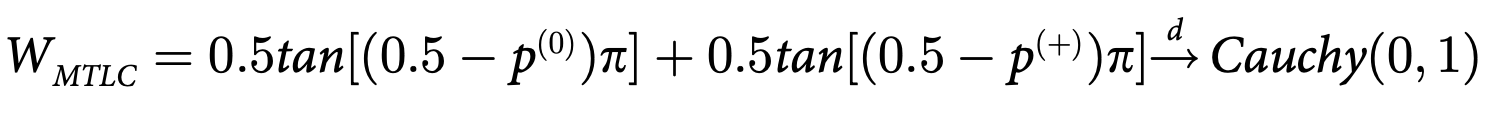
\includegraphics[width = \textwidth]{cauchy.png}
%   \end{itemize}
%
% \end{frame}
%--- Next Frame ---%

% \begin{frame}[t]{Estimating correlation coefficients }
%   \begin{itemize}
%     \item Estimated values of correlation coefficients $\hat{\boldsymbol\rho}^{(0)}$ and $\hat{\boldsymbol\rho}^{(+)}$ may be different.
%     \item When Pearson correlations are available to compute, the GEE estimates are similar.
%   \end{itemize}
% \end{frame}






\end{document}
